% Appendices file. here, cover all topics related to thesis.



\section{Performance Metrics}
The concept of verifying accuracy in a statistical estimate is covered in [xx source], and some of this information is covered briefly below. In the field of image recognition, one particularly interesting metric is "Intersection over Union", also referred to as IOU or Jaccard Index. From this metric, precision and recall may then be calculated. Precision and recall are fundamental in obtaining more abstracted metrics such as Average Precision and mean Average Precision (mAP), which are how different networks are compared. The following information is primarily taken from the well-known PASCAL VOC (visual objects classes) Challenge \cite{everingham_pascal_2010} and "An Introduction to Information Retrieval" \cite{Manning:2008:IIR:1394399}.

\subsection{Defining a Result}
The first step in measuring performance is categorizing what a result may be. With a visual task such as object classification, there are 4 possible outcomes, as shown below. In general, there may be a True Positive, False Positive, True Negative, or False Negative. In practice, True Negatives are not used, and the remaining three are used to varying degrees. Each is better clarified as such:
\begin{itemize} \itemsep=-.5em
	\item True Positive: Correctly detecting a true object
	\item False Positive: Incorrectly detecting something that isn't there
	\item False Negative: Incorrectly ignoring a true object
	\item True Negative: Correctly ignoring something that isn't there
\end{itemize}

\begin{figure}[h] % h = "approx here", {h,t,b}
	\centering
	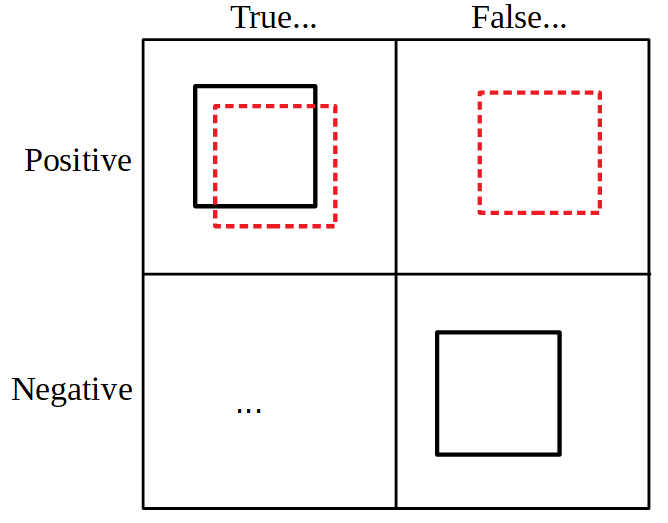
\includegraphics[width=.4\textwidth]{../media/tp_help.png}
	\caption{A visual representation of various outcomes, ground truths as solid black boxes and detections as dotted red boxes. True positives (TP) are a correct detection, FP's are a detection of no actual object, and FN's are a lack of detection of an actual object.}
	\label{tp_help} %label goes last
\end{figure}

To actually classify a result in one of these categories, computer vision depends on using the overlap of a given bounding box estimate with a bounding box ground truth. If the overlap is above some threshold, the estimate is said to be a true positive. In some metrics, two estimates overlapping the same ground truth will only count the larger overlap, or the more confident estimate. Overlap is formally known as Intersection over Union, or IOU value.

\subsection{Intersection Over Union}
In image recognition, as well as other spatially-based tasks, accuracy is needed in various forms to know "how well" a prediction overlaps, or matches, the ground truth. If, for example, an object-detection algorithm predicts the location of a car in a photo, one would like to know if such an estimate has any value, ideally with as few parameters as possible.

In light of this, Intersection Over Union encompasses all relevant aspects of rating the overlap of two geometric shapes (e.g. rectangles) while enabling an intuive, non binary scoring of an estimate. IOU is calculated as the ratio of two bounding regions' intersection over their union, as the name states. Visually, this looks something like the below in Figure \ref{iou_img}. Uniquely, the calculation of area and intersection for image boundaries is inclusive of the bounds, meaning that the length of a given difference must have ``+1" added to it. This is explained in the example below.

\begin{figure}[ht] % h = "approx here", {h,t,b}
    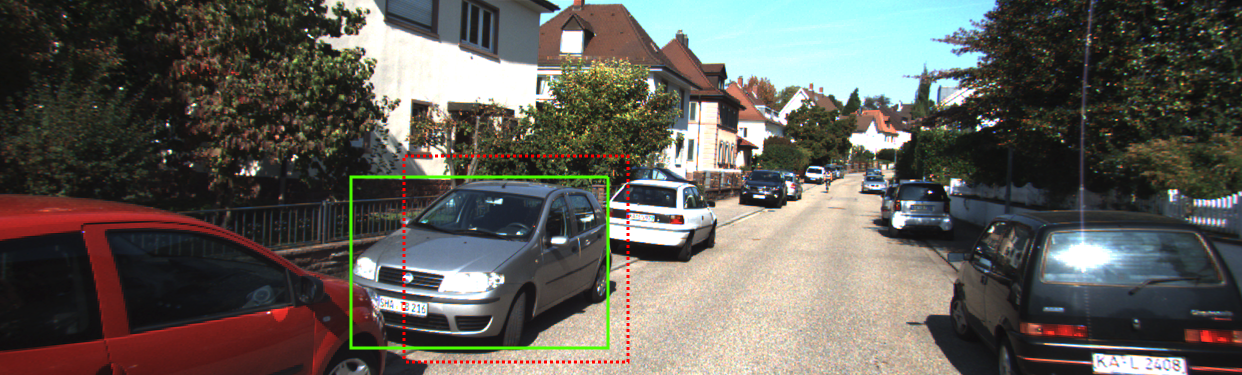
\includegraphics[width=1\textwidth]{../media/iou_img.png}
    \caption{Example of ground truth bounding box (solid green) and prediction bounding box (dashed red). In this image, the overlap between the green and red regions is the intersection, while the combined area is the union. The IOU of the two boxes is 0.64. Image index: 8.}
    \label{iou_img} %label goes last
\end{figure}

In order to formally calculate IOU, a generalized form may be generated to apply to n-dimensions. The generalized mathematical equation is simply as follows. Given a region A and a region B: 
\begin{equation}
IOU = \frac{|A\cap B|}{|A\cup B|} = \frac{|A\cap B|}{|A|+|B|- |A\cap B|}
\end{equation}

To assist in understanding IOU, a code snippet as well as an example are presented.

All aspects of calculating the IOU (including area and intersection) are broken up into multiple pieces, but presented together below. For n-dimensions, the code (presented here in python) is as follows: 


KJG190618: NEED TO RE-PASTE IN THIS CODE!!! XX
\begin{figure}[H]
\setstretch{0.84} % want code to be nice and compact
\begin{lstlisting}
import numpy as np

def extent(box,inclusive=False):
    '''
    Return the size / "extent" (length, area, volume, etc) of a given box in
        n-dimensions.
    INPUTS:
        box: n-dimensional bounds, format [x1,y1,z1, .. ,x2,y2,z2, ..]
        inclusive: boolean. add 1 unit to each dimension, such as for images
    OUTPUT:
        extent: size of box bounds, scalar float.
    '''
    o= 1 if(inclusive) else 0 # add '1' if inclusive is true
    b=np.array(box).reshape((2,-1)).T # now in internal convention
    return np.product([i[1]-i[0]+o for i in b])

def intersection(box1,box2,inclusive=False):
    '''
    Return the size / "extent" of intersection between two bounds of
        n-dimension. Internal convention follows same as "extent" function.
    INPUTS:
        box1,box2: n-dimensional bounds, format [x1,y1,z1, .. ,x2,y2,z2, ..]
        inclusive: boolean. add 1 unit to each dimension, such as for images
    OUTPUT:
        intersection: size of overlapping bounds, scalar float.
    '''
    o= 1 if(inclusive) else 0 # add '1' if inclusive is true
    b1=np.array(box1).reshape((2,-1)).T
    b2=np.array(box2).reshape((2,-1)).T # internal convention
    c=np.stack((b1,b2),2)
    # for each dimension, get (min(upperbound)-max(lowerbound)) and get product
    val = np.product([np.min(c[i,1,:])-np.max(c[i,0,:])+o for i in range(len(b1))])
    return max(val,0.0)

def IOU(b1,b2,inclusive=False):
    '''
    Return generalized intersection over union for two bounding boxes of 
        matching n-dimension.
    INPUTS:
        b1,b2: n-dimensional bounding boxes, format [x1,y1,z1, .. ,x2,y2,z2, ..]
    OUTPUT:
        iou: intersection over union, scalar float, range [0,1].
    '''
    inter = intersection(b1,b2,inclusive)
    union = extent(b1,inclusive)+extent(b2,inclusive)-inter
    return inter / union

\end{lstlisting}
\onehalfspacing % set line spacing back to normal
\caption{Python implementation of generalized IOU calculation.}
\label{code_iou}
\end{figure}

\subsubsection{Example: IOU of a Ground Truth and Prediction Label}
Suppose there is an image, as given below, where there is a ground truth label `gt' and a prediction label `pred' with 2D bounding boxes formatted as \texttt{[x1,y1,x2,y2]}, all units in pixels. To determine the IOU of the image, the calculations are listed below. Because boxes represent pixel values, remember to add "1" to each dimension.



\def \pxpx {\; [px^2]}
\def \Asub #1{A\textsubscript{#1}}
\begin{enumerate}\itemsep=-0.5em

\item Find area of each bounding box: \\ $\Asub{gt} = (x2-x1+1)*(y2-y1+1) = 16,335 \pxpx $ , $ \Asub{pr} = 12905 \pxpx $

\item Find overlapping area, e.g. intersection (see \ref{code_iou} for more info): $I = 11455 \pxpx $

\item Calculate IOU: $\frac{I}{\Asub{gt} + \Asub{pr} - I} = 0.644 $
\end{enumerate}

\begin{figure}[h] % h = "approx here", {h,t,b}
    \centering
    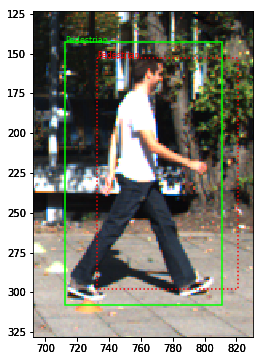
\includegraphics[width=.4\textwidth]{../media/iou_example.png}
    \caption{IOU calculation example. Ground truth (green solid) has BB: [712,143,810,307]. Prediction (red dotted) has BB: [732,153,820,297]. IOU is 0.644.}
    \label{iou_example} %label goes last
\end{figure}


\subsection{Precision \& Recall}
Once all detections have been tallied and placed into their correct categories, their precision and recall may be calculated. In information retrieval, precision is defined as "the fraction of retrieved documents that are relevant", and recall is defined as "the fraction of relevant documents that are retrieved". Reworded for object detection: precision is the number of correct predictions divided by the total number of predictions, and recall is the number of correct predictions divided by the total number of possible answers. These two are also given as equations in terms of true positives and so on. 

\begin{equation}
Precision = \frac{TruePositives}{TruePositives + FalsePositives}
\end{equation}

\begin{equation}
Recall = \frac{TruePositives}{TruePositives + FalseNegatives}
\end{equation}

In practice, the precision and recall of each detection is generated procedurally as each detection is compared to ...

KJG190618: NEED TO PERSONALLY RUN THROUGH A SIMPLE EXAMPLE OF PRECISION / RECALL, AND PUT THIS INTO YOUR PYTHON SANDBOX XX

% SAMPLE =======================================================================

\section{Sample Appendix}
TextHere

\begin{figure}[h] % h = "approx here", {h,t,b}
    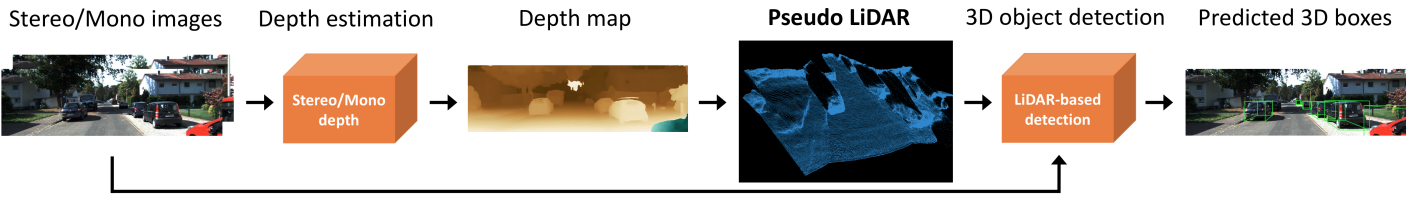
\includegraphics[width=1\textwidth]{../media/wang_pipeline.png}
    \caption{texthere}
    \label{delme_figure} %label goes last
\end{figure}


\begin{figure}[h] %h=here,t=top,b=bottom,H=exactlyHere
\setstretch{0.84} % want code to be nice and compact
% note: optional line numbers argument
\begin{lstlisting}[numbers=left]
def pyt(a,b):
    return (a**2+b**2)**0.5
\end{lstlisting}
\onehalfspacing % set line spacing back to normal
\caption{Python implementation of generalized IOU calculation.}
\label{delme_code} % label goes last
\end{figure}

%\begin{enumerate}\itemsep=-0.5em
%	\item one
%	\item two
%	\item three
%\end{enumerate}
